% Options for packages loaded elsewhere
\PassOptionsToPackage{unicode}{hyperref}
\PassOptionsToPackage{hyphens}{url}
%
\documentclass[
]{book}
\title{ResNet Data Portal User Guide}
\author{}
\date{\vspace{-2.5em}}

\usepackage{amsmath,amssymb}
\usepackage{lmodern}
\usepackage{iftex}
\ifPDFTeX
  \usepackage[T1]{fontenc}
  \usepackage[utf8]{inputenc}
  \usepackage{textcomp} % provide euro and other symbols
\else % if luatex or xetex
  \usepackage{unicode-math}
  \defaultfontfeatures{Scale=MatchLowercase}
  \defaultfontfeatures[\rmfamily]{Ligatures=TeX,Scale=1}
\fi
% Use upquote if available, for straight quotes in verbatim environments
\IfFileExists{upquote.sty}{\usepackage{upquote}}{}
\IfFileExists{microtype.sty}{% use microtype if available
  \usepackage[]{microtype}
  \UseMicrotypeSet[protrusion]{basicmath} % disable protrusion for tt fonts
}{}
\makeatletter
\@ifundefined{KOMAClassName}{% if non-KOMA class
  \IfFileExists{parskip.sty}{%
    \usepackage{parskip}
  }{% else
    \setlength{\parindent}{0pt}
    \setlength{\parskip}{6pt plus 2pt minus 1pt}}
}{% if KOMA class
  \KOMAoptions{parskip=half}}
\makeatother
\usepackage{xcolor}
\IfFileExists{xurl.sty}{\usepackage{xurl}}{} % add URL line breaks if available
\IfFileExists{bookmark.sty}{\usepackage{bookmark}}{\usepackage{hyperref}}
\hypersetup{
  pdftitle={ResNet Data Portal User Guide},
  hidelinks,
  pdfcreator={LaTeX via pandoc}}
\urlstyle{same} % disable monospaced font for URLs
\usepackage{longtable,booktabs,array}
\usepackage{calc} % for calculating minipage widths
% Correct order of tables after \paragraph or \subparagraph
\usepackage{etoolbox}
\makeatletter
\patchcmd\longtable{\par}{\if@noskipsec\mbox{}\fi\par}{}{}
\makeatother
% Allow footnotes in longtable head/foot
\IfFileExists{footnotehyper.sty}{\usepackage{footnotehyper}}{\usepackage{footnote}}
\makesavenoteenv{longtable}
\usepackage{graphicx}
\makeatletter
\def\maxwidth{\ifdim\Gin@nat@width>\linewidth\linewidth\else\Gin@nat@width\fi}
\def\maxheight{\ifdim\Gin@nat@height>\textheight\textheight\else\Gin@nat@height\fi}
\makeatother
% Scale images if necessary, so that they will not overflow the page
% margins by default, and it is still possible to overwrite the defaults
% using explicit options in \includegraphics[width, height, ...]{}
\setkeys{Gin}{width=\maxwidth,height=\maxheight,keepaspectratio}
% Set default figure placement to htbp
\makeatletter
\def\fps@figure{htbp}
\makeatother
\setlength{\emergencystretch}{3em} % prevent overfull lines
\providecommand{\tightlist}{%
  \setlength{\itemsep}{0pt}\setlength{\parskip}{0pt}}
\setcounter{secnumdepth}{5}
\usepackage{booktabs}
\ifLuaTeX
  \usepackage{selnolig}  % disable illegal ligatures
\fi
\usepackage[]{natbib}
\bibliographystyle{apalike}

\begin{document}
\maketitle

{
\setcounter{tocdepth}{1}
\tableofcontents
}
\hypertarget{overview}{%
\chapter{Overview}\label{overview}}

The ResNet Data Portal was developed using \href{https://geonode.org/}{GeoNode}, an open-source platform for sharing geospatial maps and data. This document is intended to summarize and supplement the official \href{https://docs.geonode.org/en/3.2.x/usage/index.html}{GeoNode Documentation}.

\hypertarget{navigation}{%
\section{Navigation}\label{navigation}}

\hypertarget{intro}{%
\chapter{Account Management}\label{intro}}

\hypertarget{registering-a-new-account}{%
\section{Registering a new account}\label{registering-a-new-account}}

To get started, navigate to data.nsercresnet.ca and click ``Register'' in the top right.

\begin{figure}
\centering
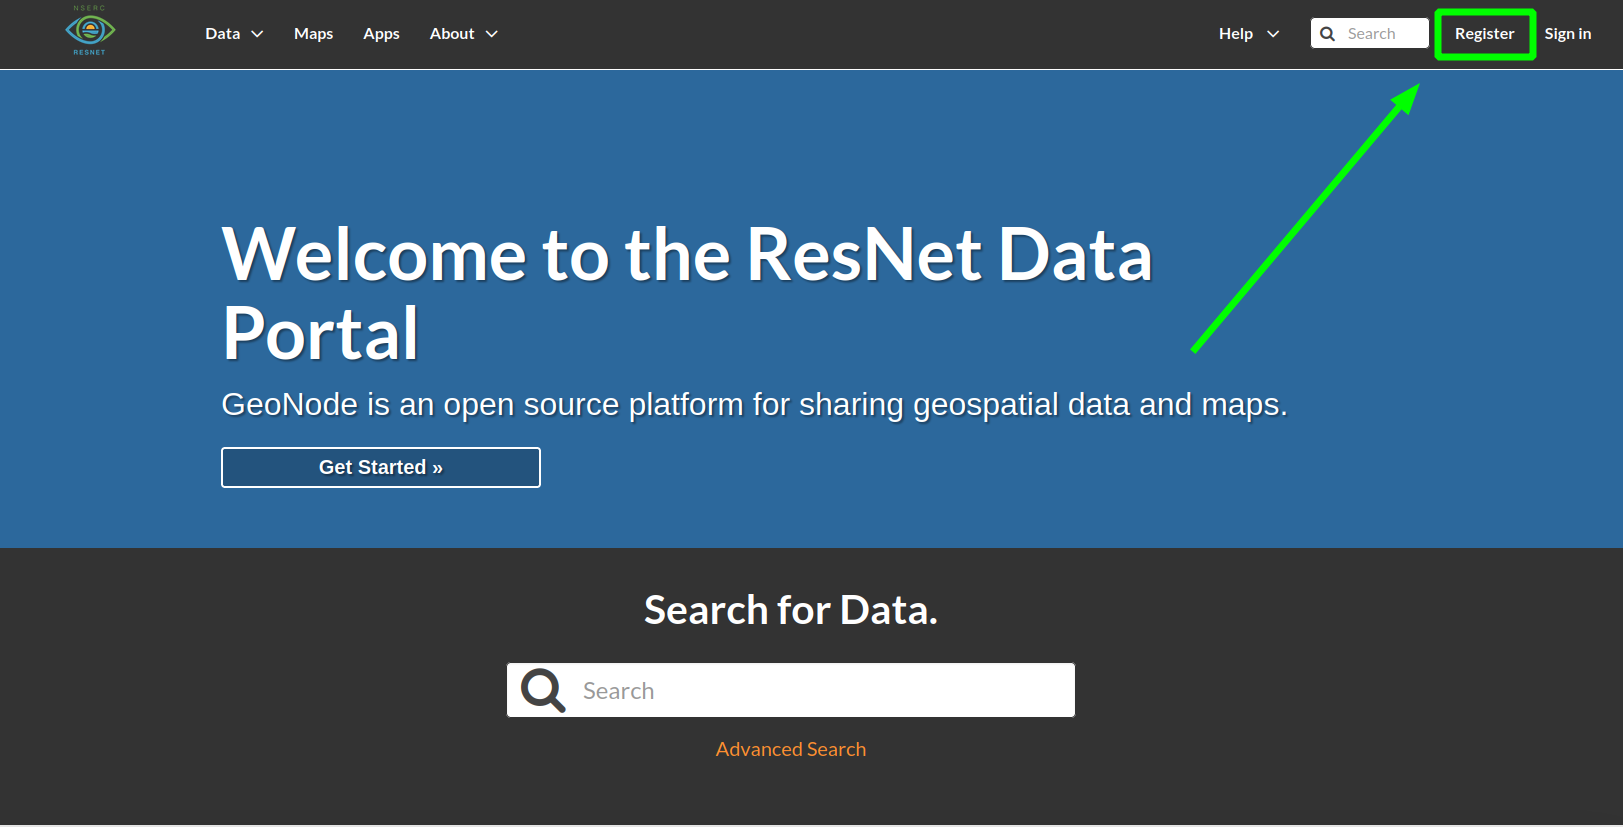
\includegraphics{images/paste-B29D8E77.png}
\caption{Registration button on Data Portal landing screen}
\end{figure}

\begin{itemize}
\tightlist
\item
  \underline{E-mail}: Address to affiliate with your account. This is where the system will send notifications.
\item
  \underline{Username}: Your username should follow the pattern \texttt{firstname.lastname} (eg \texttt{john.clark}).
\item
  \underline{Password}: Create a strong password unique to this account. Consider using a password manager like \href{https://bitwarden.com/}{Bitwarden}.
\end{itemize}

Email notifications are sent from \texttt{resnet.data.portal@gmail.com}. Remember to check your spam folder!

\protect\hyperlink{navigation}{Navigation}

\hypertarget{updating-your-profile}{%
\section{Updating your profile}\label{updating-your-profile}}

\hypertarget{joining-a-group}{%
\section{Joining a group}\label{joining-a-group}}

\hypertarget{data-layers}{%
\chapter{Data Layers}\label{data-layers}}

\hypertarget{uploading-a-new-layer}{%
\section{Uploading a new layer}\label{uploading-a-new-layer}}

\hypertarget{styling-layers}{%
\section{Styling layers}\label{styling-layers}}

\hypertarget{publishing-layers}{%
\section{Publishing layers}\label{publishing-layers}}

\hypertarget{maps}{%
\chapter{Maps}\label{maps}}

\hypertarget{creating-maps}{%
\section{Creating maps}\label{creating-maps}}

\hypertarget{embedding-maps}{%
\section{Embedding maps}\label{embedding-maps}}

\hypertarget{metadata}{%
\chapter{Metadata}\label{metadata}}

\hypertarget{getting-help}{%
\chapter{Getting Help}\label{getting-help}}

\hypertarget{slack}{%
\section{Slack}\label{slack}}

\hypertarget{request-support}{%
\section{Request Support}\label{request-support}}

\hypertarget{external-resources}{%
\section{External Resources}\label{external-resources}}

  \bibliography{book.bib,packages.bib}

\end{document}
